% !TeX program = lualatex
\PassOptionsToPackage{dvipsnames}{xcolor}
\documentclass[9pt]{beamer}

\geometry{paperwidth=213.3mm,paperheight=120mm}

\usetheme[{titleformat plain}=smallcaps,
           titleformat title=smallcaps,
           titleformat subtitle=regular,
           titleformat section=smallcaps,
           titleformat frame=smallcaps,
           % numbering=fraction,
          ]{metropolis}
% \usepackage{appendixnumberbeamer}

\usepackage{../_style/common}
\usepackage{../_style/defs}

\definecolor{mLightGreen}{HTML}{14B03D}
\definecolor{vpGreen}{HTML}{66c2a5}
\definecolor{vpOrange}{HTML}{fc8d62}
\providecommand{\iRef}[1]{{\color{mLightGreen}\small $[$#1$]$}}
\hypersetup{urlcolor=mLightGreen}

\usepackage{alphalph}

\usepackage{enumitem}
\setenumerate[1]{%
      label=\protect\usebeamerfont{enumerate item}%
      \protect\usebeamercolor[fg]{enumerate item}%
      \insertenumlabel.}
\setitemize{label=\usebeamerfont*{itemize item}%
    \usebeamercolor[fg]{itemize item}
      \usebeamertemplate{itemize item}}

\graphicspath{{pictures/}{../_pictures/}{../2022-Gargnano/pictures/}}

\usepackage[symbol]{footmisc}
\renewcommand{\thefootnote}{\fnsymbol{footnote}}
\renewcommand{\phantom}{\textsc{Phantom}\xspace}
\newcommand{\sphluid}{\texttt{sphluid}\xspace}
\newcommand{\sphlash}{\texttt{sphlash}\xspace}

\title{Fluid dynamics Exam}
\subtitle{
    DS Tau hidden planet \href{https://arxiv.org/abs/2005.04244}{arXiv:2005.04244} \&\\
    Proposals for simulations refactoring
}
\date{November, 2022}
\author{Alessandro Candido \& \textsc{NNPDF}}
%\institute{N3PDF}
\titlegraphic{
    \vspace*{10pt}
    \hfill
\includegraphics[height=1.5cm]{../_logos/unimi_logo.png}\hspace*{1cm}
}

\begin{document}

\maketitle

\setlist[description]{font=\quad\normalfont\bfseries\scshape\space}
\metroset{block=fill}

\section{DS Tau \iRef{\href{https://arxiv.org/abs/2005.04244}{2005.04244}}}

\begin{frame}[fragile]{Something}
    \begin{columns}
        \begin{column}{0.5\textwidth}
        \end{column}
        \begin{column}{0.5\textwidth}
            \begin{lstlisting}[language=yaml, style=mystyle, breaklines=true]
description: |
  explain parameters in 'dustydisc.setup'

schema:
  $variable:
    value: the chosen value
    motivation: reason for the choice
    position: |
      searchable reference in arxiv:2005.04244 [...]

parameters:
  # resolution
  np:
    value: 300000
    motivation: |
      enough resolution, without pushing to much performances
    position: null

  # central object(s)/potential
  icentral:
    value: 1
    motivation: |
      the central star is modeled as a sink particle
    position: |
      We model the planet and the central star as sink particle\end{lstlisting}
        \end{column}
    \end{columns}
\end{frame}

\section{Simulations Proposals}

\begin{frame}{Motivation}
    \begin{columns}
        \begin{column}{0.5\textwidth}
            This part is here to motivate a design work that I've done in the
            process to write my own simulation tool.

            \vspace*{10pt}
            \begin{center}
                \githuburl{https://github.com/AleCandido/sphluid}
            \end{center}


            \vspace*{20pt}
            \begin{alertblock}{Disclaimer}
                This repository is not well-maintained, and some notes
                (including top-level \texttt{README.md}) do not represent the
                most recent status of investigation.

                {\footnotesize
                    Most of the work focused on the engine,
                    \href{https://github.com/AleCandido/sphluid/tree/main/sphluid}{\sphluid}.
                    Though still incomplete, the design was quite advanced, and
                    will be discussed here.
                    One of the more relevant pieces is actually the
                    \href{https://github.com/AleCandido/sphluid/blob/72b9c26eeb969915933ccd50a793b5244255e68a/sphluid/Cargo.toml\#L19-L27}{list
                    of dependencies}.
                }
            \end{alertblock}
        \end{column}
        \begin{column}{0.5\textwidth}
            The idea of the project was to start from some \textbf{basic} (but
            non-trivial) \textbf{physics}, and try to \textbf{reduce} the
            \alert{\textbf{development effort}}.
            \vspace*{30pt}

            \textsc{\color{BrickRed} \textbf{Cons}}:
            \begin{itemize}
                \item the goal is physics, not development
                \item refactoring takes a lot of time, to obtain a result that
                  was already there
            \end{itemize}
            
            \textsc{\color{mLightGreen} \textbf{Pros}}
            \begin{itemize}
                \item refactoring
                \begin{itemize}
                    \item might improve performances, or other technical features
                    \item nothing is perfect at the first shot, iterating is required
                    \item drastically \textbf{reduce implementation time} of
                      new features
                \end{itemize}
                \item software evolves fast, and new tools can open new options
            \end{itemize}
        \end{column}
    \end{columns}
\end{frame}

\begin{frame}{Technology}
    \begin{columns}
        \begin{column}{0.5\textwidth}
            One of the most apparent differences between \phantom and \sphluid
            is the programming language.

            \vspace*{5pt}
            \begin{table}
                \centering
                \hspace*{-15pt}
                \begin{tabular}{cc}
                    \phantom & \sphluid\\
                    \noindent\parbox[c]{0.5\hsize}{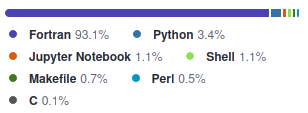
\includegraphics[width=0.48\textwidth]{langs-phantom}} &
                    \noindent\parbox[c]{0.5\hsize}{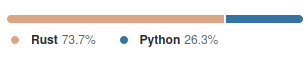
\includegraphics[width=0.48\textwidth]{langs-sphluid}}
                \end{tabular}
            \end{table}
            \vspace*{10pt}

            Nevertheless, the \textit{bare language} itself is not the most
            relevant difference, but instead the
            \textit{\textbf{\alert{tooling}}} that comes with the language is
            extremely relevant.
        \end{column}
        \begin{column}{0.5\textwidth}
            \begin{tabular}{m{0.45\hsize}|m{0.45\hsize}}
                \textbf{Fortran and C} & \textbf{Rust}\\
                \hline
                Require external build system &
                Provided and widespread\\
                \texttt{Makefile} manual and needs files (further code) &
                \texttt{cargo} based on conventions\\
                manual dependency management (or meta-build tools) &
                automated \& declarative\\
                many Linux distribution + further repos &
                official package registry, \url{crates.io}\\
                \dots & \dots
            \end{tabular}
            
            \vspace*{15pt}
            More language are available (linter, formatter, static analysis,
            \dots) that help development.
            And modern language features (enums $\sim$ algebraic data types,
            pattern matching, memory safety, \dots) are also useful features.

            \vspace*{15pt}
            But the main point I want to stress is about the \textbf{dependency
            management}.
        \end{column}
    \end{columns}
\end{frame}

\begin{frame}{Dependencies}
    \begin{columns}
        \begin{column}{0.5\textwidth}
            \vspace*{20pt}
            \begin{figure}
                \centering
                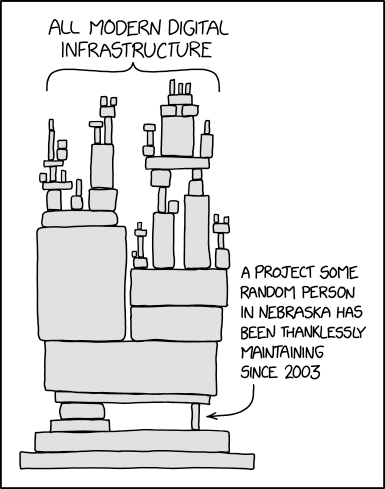
\includegraphics[width=0.7\textwidth]{dependency}
                \caption{
                    xkcd \enquote{Dependency} cartoon,
                    \url{https://xkcd.com/2347/}
                }
            \end{figure}
        \end{column}
        \begin{column}{0.5\textwidth}
            \begin{center}
                \itshape
                Dependencies are complex, and they may cause a lot of troubles.
            \end{center}

            Still, there are reliable dependencies, and they can
            \alert{\textbf{factorize}} a lot of work.
            They are well-known in Python ecosystem:
            \begin{itemize}
                \item data structures $\to$ NumPy 
                \item scientific computation $\to$ SciPy
                \item plotting $\to$ Matplotlib
                \item Machine Learning $\to$ TensorFlow + PyTorch + \dots
                \item serialization $\to$ PyYAML (or built \texttt{json})
                \item \dots
            \end{itemize}

            In C/C++ and Fortran, while not missing reliable libraries (for
            some dedicated goals), there was the \textbf{distribution problem}.

            Two solutions were available for portability: meta-build systems
            (autotools, CMake, Meson, \dots) and static compilation.
            But both cases had complications in distribution $\to$ the birth of
            Linux \textbf{package managers}.

            \begin{block}{Update}
                Today there are modern solutions also for those ecosystems: Git
                submodules and containers are motivated also by these issues.
            \end{block}
        \end{column}
    \end{columns}
\end{frame}

\begin{frame}[fragile]{\sphluid dependencies}
    \begin{columns}
        \begin{column}{0.5\textwidth}
            \vspace*{15pt}

            The following is the list of the dependencies for the \sphluid
            crate:
            \begin{lstlisting}[language=ini, style=mystyle, breaklines=true]
[dependencies]
anyhow = "1.0.42"
itertools = "0.10.5"
ndarray = "0.15.3"
netcdf = { version = "0.7.0", features = ["static"] }
numpy = "0.16.2"
pyo3 = { features = ["extension-module", "multiple-pymethods"], version = "0.16.4" }
rand = "0.8.4"
rayon = "1.5.1"\end{lstlisting}
        \vspace*{10pt}

            The first point to remark, it is that this is contained in the file
            \href{https://github.com/AleCandido/sphluid/blob/main/sphluid/Cargo.toml}{\texttt{Cargo.toml}},
            and fully replaces the \texttt{Makefile}, including features of
            meta-build tools.

            Leveraging conventions, these files are extremely simple, and
            purely declarative\footnote{
                This one is 27 lines, at the time of writing, containing mostly
                package metadata and dependencies.
            }.

            All packages are available at \url{https://crates.io}, with the
            name they are cited.
            \vspace*{10pt}
        \end{column}
        \begin{column}{0.5\textwidth}
            What are actually they doing?
            \begin{itemize}
                \item \texttt{ndarray} provides a full-fledged
                  \alert{\textbf{array structure}} (the Rust equivalent of
                  NumPy)
                \item \texttt{rayon} gives an iterator that automatically
                  parallelize (on CPU) the operation executed (specified with
                  a closure)
                \item \texttt{netcdf} crate provides handlers for the netCDF4
                  file format, an appendable file format (based on HDF5) to
                  store a set of multidimensional array, possibly sharing
                  coordinates (developed by the weather and climate community)
                \item \texttt{pyo3} provides an extremely is way to generate
                  \alert{\textbf{Python bindings}} (FFI), and \texttt{numpy}
                  crate extend the mapping to \texttt{ndarray}
                  $\leftrightarrow$ NumPy
                \item \texttt{anyhow} simplifies native exception management,
                  \texttt{itertools} provides useful iterators, \texttt{rand}
                  is an RNG library
            \end{itemize}
        \end{column}
    \end{columns}
\end{frame}

\begin{frame}{Setup \& Architecture}
    \begin{columns}
        \begin{column}{0.5\textwidth}
            \vspace*{15pt}

            Initially, I started designing the setup functions as a
            \textbf{series of possible configurations}, with optional
            parameters.

            This is the strategy adopted by \phantom
            \vspace*{10pt}

            While this is certainly a possible way to do it, it has some
            drawbacks:
            \begin{itemize}
                \item an \textbf{extensive set} of conditions has to be provided
                \item as time passes, they will \textbf{get more complicate},
                    so more configurations will be needed
                \item when a complex configuration does not foresee a possible
                  use case, the code of the \textbf{configuration has to be
                  patched} to allow it
                  \begin{itemize}
                      \item \textbf{less} people are \textbf{able to write} the
                        program \textbf{than} those who are \textbf{running} it
                      \item more people will have to patch the code: harder to
                        \textbf{manage contributions}
                  \end{itemize}
            \end{itemize}
            \vspace*{10pt}

            \textbf{\textsc{\color{ForestGreen} Counterproposal}}: write a
            \alert{\textbf{setup library}} and short example programs to create
            some configurations.

            This has the advantage of allowing at least one more data type to
            be passed: \alert{\textbf{functions}} (i.e.\ code).
            
            It is extremely flexible, since functions can be
            \textit{\textbf{composed}}, and \textbf{\textit{mathematical
            expressions}} can also be encoded as functions.
        \end{column}
        \begin{column}{0.5\textwidth}
            \begin{figure}[T]
                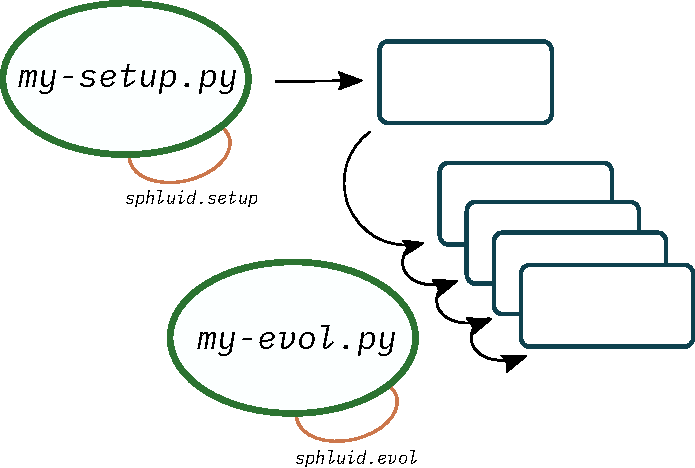
\includegraphics[width=0.8\hsize]{sphluid-arch}
                \caption{
                    Current design for \sphluid architecture.
                }
            \end{figure}

            Because of efficiency requirements, the libraries will be written
            in Rust, but the simple driver programs will be written in Python,
            that is a far more accessible language (reflecting the different
            audience).
            \vspace*{10pt}

            The same model is repeated for the evolution part, for which only
            the evolution step will be done in Rust, but the rest of the
            management will be Python (and as simple as possible).
        \end{column}
    \end{columns}
\end{frame}

\begin{frame}{Analysis}
    \begin{columns}
        \begin{column}{0.5\textwidth}
            The analysis will be done in Python as well, where all the
            libraries to manage the dumps are already available.

            The custom part of the file format (the dump format, built on top
            of some other standard like netCDF4) will be in
            \texttt{sphluid.io}, and available to reuse also in the analysis
            code.
            \vspace*{10pt}

            The analysis framework will leverage all the huge availability of
            tools in Python:
            \begin{itemize}
                \item data structures: NumPy, Pandas, Xarray
                \item scientific computing: Scipy
                \item notebook programming: Jupyter (Notebook/Lab)
                \item machine learning (why not?): Scikit-Learn, TensorFlow
            \end{itemize}
        \end{column}
        \begin{column}{0.5\textwidth}
            Reusable tools will be collected into another library, this time
            pure Python: \sphlash.

            \begin{center}
                \centericon{github}~\href{https://github.com/AleCandido/sphluid/tree/main/sphlash}{AleCandido/sphluid/sphlash}
            \end{center}

            Also this libraries can accept contributions from a wider audience,
            splitting the contributor role from low-level development (high
            performances or graphics).
        \end{column}
    \end{columns}
\end{frame}


\begin{frame}[standout]
    Thanks for your attention!
\end{frame}

\begin{frame}{Something}
    \begin{columns}
        \begin{column}{0.5\textwidth}
        \end{column}
        \begin{column}{0.5\textwidth}
        \end{column}
    \end{columns}
\end{frame}

% \appendix

\end{document}
